\documentclass{beamer}
\usetheme{Warsaw}
\useinnertheme{circles}
\useoutertheme[subsection=false]{smoothbars}
\usepackage[utf8x]{inputenc}
\usepackage[czech]{babel}
\usepackage[T1]{fontenc}
\usepackage{listings}
\usepackage{tikz}
\lstset{basicstyle=\tiny\ttfamily}
\logo{
\includegraphics[height=0.5cm]{brmlab.pdf}}

\begin{document}

\AtBeginSection[]
{
  \begin{frame}
    \frametitle{Outline}
    \tableofcontents[currentsection]
  \end{frame}
}

\title{brmiversity: Umělá inteligence \\ a teoretická informatika}
\subtitle{Přednáška č. 5}
\author{Petr Baudiš $\langle${\tt pasky@ucw.cz}$\rangle$}
\institute{
	brmlab 2011\\
	\vskip 1ex
	\pgfdeclareimage[height=4ex]{ccbysa}{by-sa.pdf}
	\pgfuseimage{ccbysa}
}
\date{}
\frame{\titlepage}

\section{Základní algoritmy}

\subsection{}
\begin{frame}{Prohledávání v grafech}
\begin{itemize}
\item Chceme projít celý graf
\item Graf může být popsaný implicitně \\ (průběh výpočtu, hry)
\item Něco {\em hledáme} --- určitý uzel (řešení), cestu, \dots
\item Hledání uzlu: BFS (prohledávání do šířky), \\ DFS (prohledávání do hloubky)
\item Nejkratší cesta: Dijkstra
\end{itemize}
\begin{tikzpicture}[remember picture,overlay]
  \node [xshift=-4.5cm,yshift=-4.5cm,above right] at (current page.north east)
    {\includegraphics[width=4cm]{graph.pdf}};
\end{tikzpicture}
\end{frame}

\subsection{}
\begin{frame}{BFS, DFS}
\begin{center}
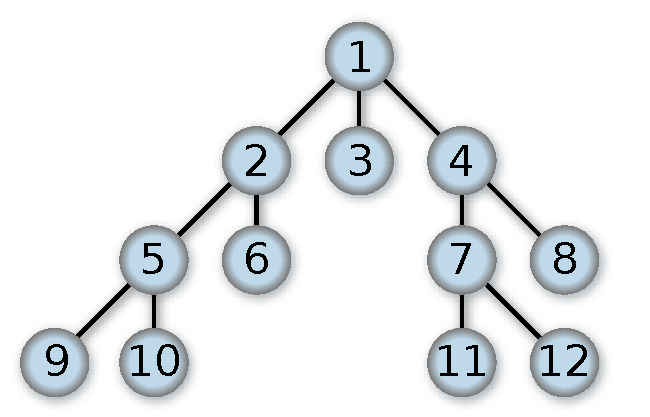
\includegraphics[width=5.5cm]{Breadth-first-tree.pdf}
\vskip 0.5ex
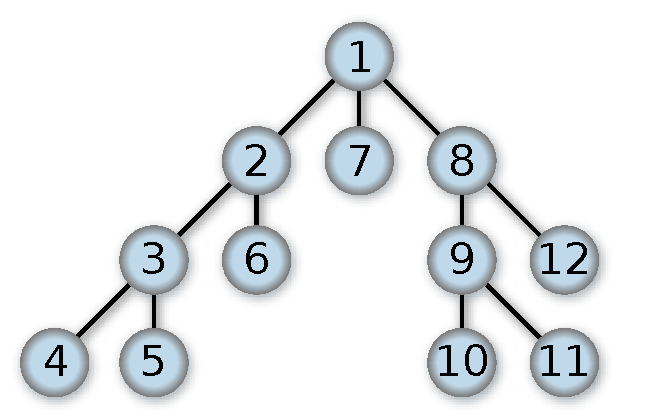
\includegraphics[width=5.5cm]{Depth-first-tree.pdf}
\end{center}
\end{frame}

\subsection{}
\begin{frame}{BFS, DFS}
\begin{itemize}
\item BFS i DFS jsou úplné; fronta LIFO nebo FIFO
\item Implicitní DFS: Backtracking, graf si nemusím držet v paměti
\item Depth-limited search
\item Iterative deepening
\item Best-first search
\item Oboustranné vyhledávání
\end{itemize}
\end{frame}

\subsection{}
\begin{frame}{Dijkstra}
\begin{itemize}
\item Budujeme strom nejkratší cesty z vrcholu do zbytku grafu
\item Vždy přidáme nejkratší hranu vedoucí ze stromu
\end{itemize}
\begin{center}
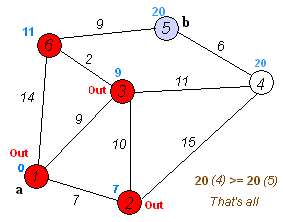
\includegraphics[width=7cm]{dijkstra.png}
\end{center}
\end{frame}

\section{Umělá inteligence a adaptivní agenti}

\subsection{}
\begin{frame}{Prohledávání v grafech}
\begin{itemize}
\item Kontext umělé inteligence?
\item Graf může být obrovský
\item Může nám stačit přibližné řešení
\item O problému máme informace navíc (heuristiky)
\vskip 3ex
\item Agent naviguje v realném prostoru reprezentovaném grafem
\end{itemize}
\end{frame}

\subsection{}
\begin{frame}{Prohledávání v grafech}
\begin{center}
A*, HPA*, PRA*, inkrementální metody
\vskip 4ex
\url{http://bajeluk.matfyz.cz/mff/algs-4-pathf.pdf}
\end{center}
\end{frame}

\subsection{}
\begin{frame}{Otázky?}
\begin{center}
Příště UI: Zpracování neurčité informace.

Příště Agenti: Komunikace a znalosti v multiagentních systémech.
\end{center}
\end{frame}

\section{Neuronové sítě}

\subsection{}
\begin{frame}{Umělá neuronová síť}
\begin{itemize}
\item Umělé neurony (``výpočetní krabičky'') \\ dostávají vstupy (čísla) a na jejich \\ základě generují výstup (číslo)
\item Obvykle: Vrstvy striktně oddělené, \\ vstupní vrstva se vstupy zvnějšku, \\ výstupní vrstva s výstupem pro uživatele, \\ skryté vrstvy vyhodnocují různé charakteristiky vstupů
\item Dnes: Více vrstev neuronů, jak je učit?
\end{itemize}
\begin{tikzpicture}[remember picture,overlay]
  \node [xshift=-4.5cm,yshift=-6cm,above right] at (current page.north east)
    {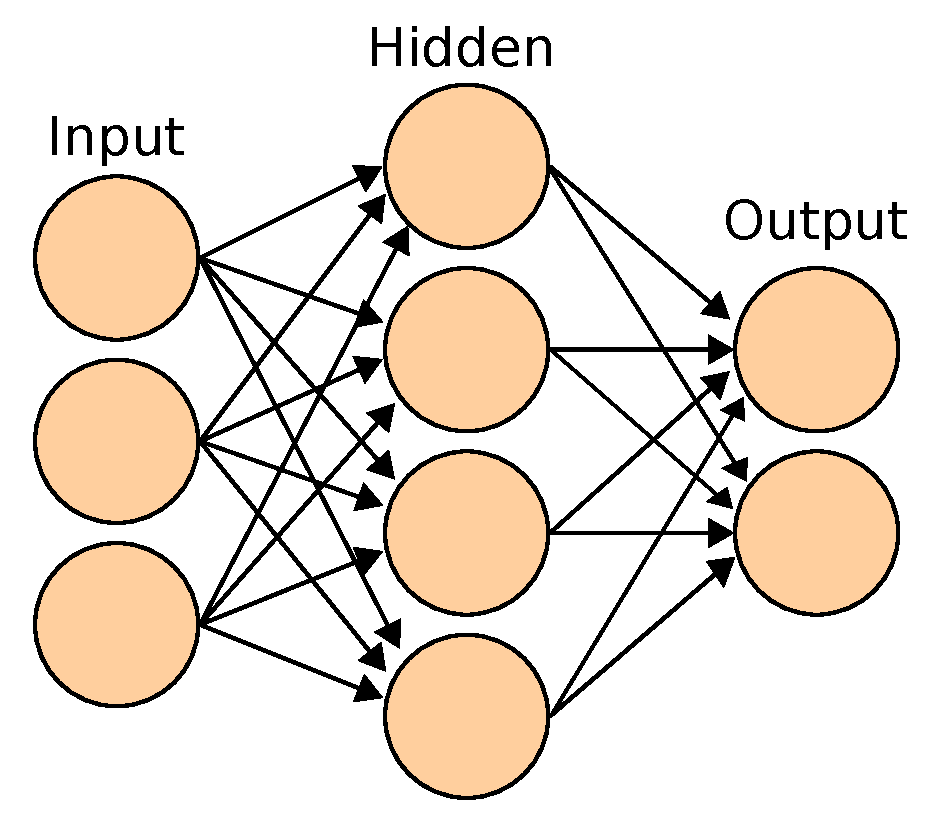
\includegraphics[width=4cm]{ANN.pdf}};
\end{tikzpicture}
\end{frame}

\subsection{}
\begin{frame}{Připomenutí: Umělý neuron}
\begin{columns}
\begin{column}{4cm}
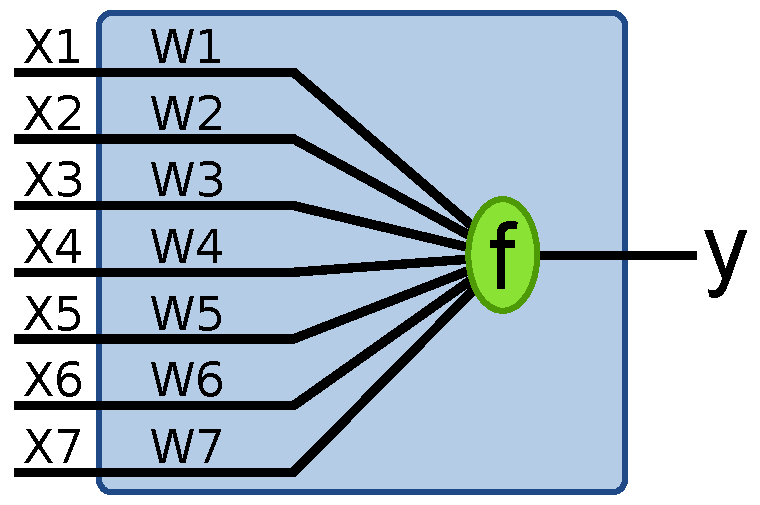
\includegraphics[width=4cm]{Perceptron.pdf}
\vskip 2ex
\includegraphics[width=4cm]{sigmoid.pdf}
\end{column}
\begin{column}{7cm}
\begin{itemize}
\item $n$ vstupů a práh $\Leftarrow$ výstup
\item Lineární kombinace --- vstupy mají různé váhy, vynásobíme, sečteme a otestujeme
\item Výstup je ``skoro'' 1/0: sigmoida
\pause
\vskip 3ex
\item Vstup $\vec x$, váhový vektor $\vec w$, práh 0
\item $\xi = \sum_{i=0}^n w_i \cdot x_i$
\item Výstupní funkce: $y = f(\xi) = {1 \over 1+e^{-\lambda\xi}}$
\end{itemize}
\end{column}
\end{columns}
\end{frame}

\subsection{}
\begin{frame}{Vícevrstvá NN}
\begin{itemize}
\item $m$ vrstev, v každé $n_m$ neuronů, propojení vždy pouze $n_i \to n_{i+1}$
\item Inicializace vstupů v první vrstvě
\item Iterativní posílání výstupů z jedné vrstvy do vstupů další vrstvy
\item Výstup poslední vrstvy je výstup celé sítě
\pause
\vskip 3ex
\item Víme, kterým vstupům mají odpovídat které výstupy
\item Vstupy a výstupy spolu však souvisejí pouze nepřímo
\item Jak odvodit konkretní váhy spojů v síti?
\end{itemize}
\end{frame}

\subsection{}
\begin{frame}{Učení vícevrstvé NN}
\begin{itemize}
\item Algoritmus zpětného šíření \\
	(existují alternativy, příliš se nepoužívají)
\item Myšlenka: Závislosti mezi vstupy a výstupy dokážeme přiměřeně matematicky popsat
\item Chceme upravit váhy podle {\em chyby}, kterou propagovaly; \\ větší váha nese větší chybu
\vskip 3ex
\item Iterujeme učení podle vstupních množin:
\begin{itemize}
\item Zjistíme chybu výstupu
\item Spočítáme {\em gradient} chyby podle vah jednotlivých spojů
\item Chybu se pokusíme zredukovat posunutím vah proti gradientu
\item Chybu ``zpětně šíříme'' do předchozí vrstvy a opakujeme
\end{itemize}
\end{itemize}
\end{frame}

\subsection{}
\begin{frame}{Derivace a gradient}
\begin{columns}
\begin{column}{5.5cm}
Derivace:

Non-free artwork.
%\includegraphics[width=5.5cm]{derivace.png}
\end{column}
\begin{column}{5.5cm}
Gradient:

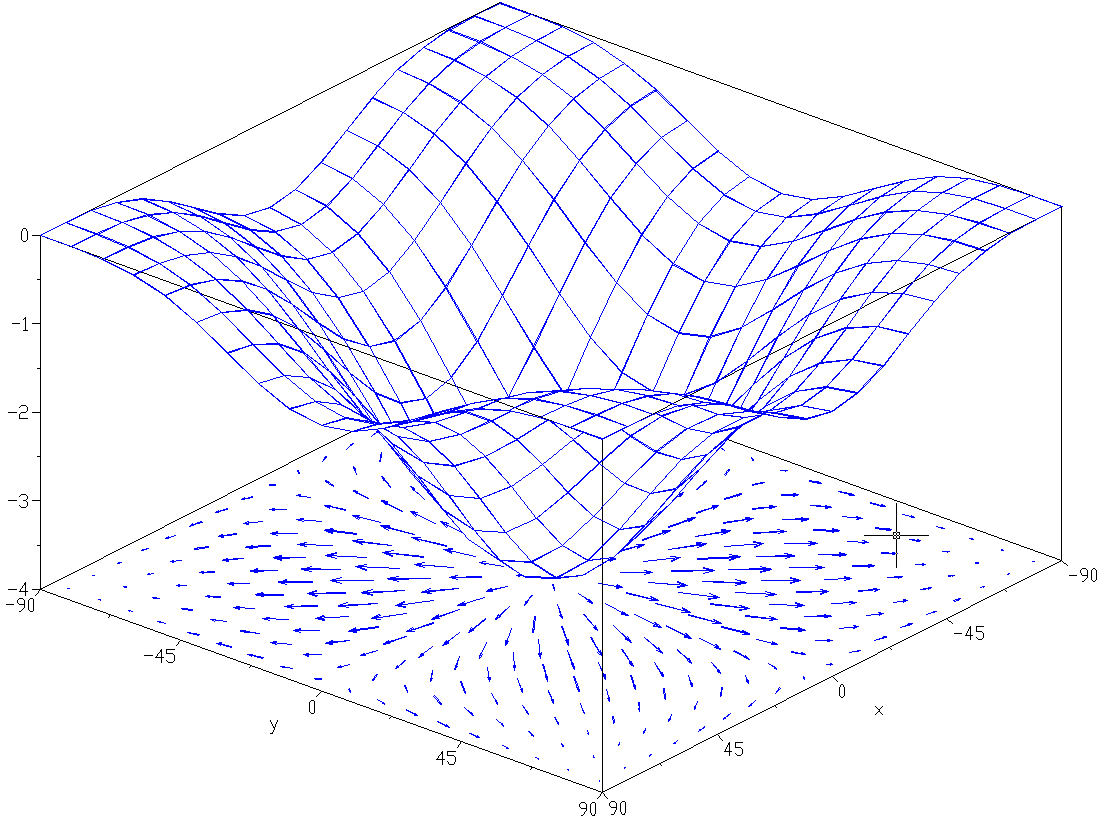
\includegraphics[width=5.5cm]{Gradient99.png}
\end{column}
\end{columns}
\end{frame}

\subsection{}
\begin{frame}{Učení poslední vrstvy}
\begin{itemize}
\item Chybová funkce: $E = {1 \over 2} \sum_p \sum_j (y_{p,j} - d_{p,j})^2$ \\
	Chceme její hodnotu {\em minimalizovat}
\item Chyba se mění podle váh neuronů (na těch závisí $y_{p,j}$) \\
	Posuneme se {\em proti} této změně:
	$\Delta_E w_{i,j} = -{\partial E \over \partial w_{i,j}}$
\end{itemize}
\pause
\vskip 2ex
$$ \xi = \sum_k w_k \cdot x_k \qquad y = f(\xi) $$
$$ \frac{\partial E}{\partial w_{i,j}} =
	\frac{\partial E}{\partial y_j} \cdot \frac{\partial y_j}{\partial \xi_j} \cdot \frac{\partial \xi_j}{\partial w_{i,j}} =
	(y_j - d_j) \cdot f'(\xi_j) \cdot y_i = \delta_i \cdot y_i $$
\pause
\vskip 2ex
Derivace sigmoidy $f'(\xi) = \left(1 \over 1+e^{-\lambda\xi}\right)' = \lambda \cdot f(\xi) \cdot (1-f(\xi))$
\end{frame}

\subsection{}
\begin{frame}{Učení vnitřních vrstev}
\begin{center}
Podobná myšlenka jako poslední vrstva, \\ jen využíváme informaci o chybě z minulé vrstvy.
\end{center}
\end{frame}

\subsection{}
\begin{frame}{Otázky?}
\begin{center}
Příště: Statistické zpracování dat, PCA.
\end{center}
\end{frame}

\section{Vyčíslitelnost}

\subsection{}
\begin{frame}{Rekapitulace}
\begin{itemize}
\item Rekapitulace: Nezajímá nás, jak rychle to poběží, \\ ale jestli to někdy doběhne.
\item Zkoumáme výpočetní {\em možnosti} algoritmů.
\vskip 3ex
\item Pro modelování výpočetních mezí \\ potřebujeme matematický popis programů.
\item Primitivně rekurzivní, obecně rekurzivní \\ a částečně rekurzivní funkce.
\end{itemize}
\end{frame}

\subsection{}
\begin{frame}{Rekurzivní funkce}
\begin{itemize}
\item Funkce: $o(x) = 0 \, \forall x$, $s(x) = x+1 \, \forall x$, $I^j_n(x_1,\ldots,x_n) = x_j$
\vskip 3ex
\pause
\item Operátor substituce: $S_n^m(f,g_1,\ldots,g_m)=h$, $h(x_1,\ldots,x_n) \simeq f(g_1(x_1,\ldots,x_n),\ldots,g_m(x_1,\ldots,x_n))$
\item Operátor prim. rekurze: $R_n(f,g)=h$, $h(0,x_2\ldots,x_n) \simeq f(x_2,\ldots,x_n)$,
	$h(i+1,x_1,\ldots,x_n) \simeq g(i, h(i,x_2,\ldots,x_n), x_2,\ldots,x_n)$
\vskip 3ex
\item Operátor minimalizace: $M_n(f) = h$, $h(x_1,\ldots,x_n) = z \Leftrightarrow f(x_1,\ldots,x_n,z)=0$ a $z$ je nejmenší
\vskip 3ex
\pause
\item {\bf Primitivně rekurzivní funkce:} Bez operátoru minimalizace.
\item {\bf Obecně rekurzivní funkce:} Na každém vstupu doběhnou.
\item {\bf Částečně rekurzivní funkce:} Mohou a nemusí doběhnout.
\end{itemize}
\end{frame}

\subsection{}
\begin{frame}{Druhy rekurzivních funkcí}
\begin{itemize}
\item {\bf Primitivně rekurzivní funkce:} Bez operátoru minimalizace.
\item {\bf Obecně rekurzivní funkce:} S minimalizací, ale každém vstupu doběhnou.
\item {\bf Částečně rekurzivní funkce:} Mohou a nemusí doběhnout.
\vskip 3ex
\pause
\item $ PRF \subset ORF \subset CRF $
\item Neostré inkluze celkem zřejmé
\item ČRF, která není ORF --- třeba minimalizace funkce $s$
\item ORF, která není PRF --- třeba univerzální funkce pro PRF
\vskip 3ex
\pause
\item Každé ČRF můžu přiřadit číslo --- na základě jejího odvození
\end{itemize}
\end{frame}

\subsection{}
\begin{frame}{Kleenova věta}
\begin{itemize}
\item {\bf Univerzální TS:} ``Emulátor'' --- vrátí výstup libovolného TS na základě jeho popisu a vstupu
\item {\bf Univerzální RF $\Psi(e,\vec x)$:} ``Emulátor'' --- vrátí výstup libovolné RF na základě jejího čísla $e$ a parametrů $\vec x$
\vskip 3ex
\pause
\item {\bf s-m-n věta:} Curryfikace RF. $\Psi(e,\vec z, \vec x) = \Psi(s(e, \vec z), \vec x)$
\vskip 3ex
\pause
\item {\bf Turingův predikát $T(e,\vec x,y)$:} Propojení s logikou, je pravdivý, pokud program $e$ s parametry $\vec x$ vrátí $y$.
\item V logice lze přes $T$ popsat ČRP, ORP, PRP (\dots predikáty).
\end{itemize}
\end{frame}

\subsection{}
\begin{frame}{Univerzální funkce}
\begin{itemize}
\item Máme univerzální ČŘF emulující jakouliv ČRF.
\item Umíme udělat univerzální PRF pro všechny PRF?
\pause
\item Neumíme. Mějme $f(e,x)$ univerzální PRF. Zavedeme PRF $g(x) = f(x,x) + 1$ s číslem $e$: $f(e,x) = g(x)$. Ale tedy $f(e,e) = g(e) = f(e,e) + 1$, což je spor.
\vskip 3ex
\pause
\item Univerzální RF pro ORF je ČRF.
\end{itemize}
\end{frame}

\subsection{}
\begin{frame}{Množiny popsané funkcemi}
\begin{itemize}
\item Množiny obvykle definujeme {\em predikáty} --- např. $\{x \,|\, x \in N,\, 5<x<10\}$
\item Predikát koresponduje k funkci
\item Tedy {\bf primitivně rekurzivní}, {\bf rekurzivní} a {\bf částečně rekurzivní} množiny, RF rozhoduje o prvku, patří-li do množiny
\item $M$ je rekurzivní, právě když je ona i doplněk rekurzivně spočetné
\end{itemize}
\end{frame}

\subsection{}
\begin{frame}{Otázky?}
\begin{center}
Příště: Věty o rekurzi a jejich aplikace.
\end{center}
\end{frame}

\subsection{}
\begin{frame}{Děkuji vám}
\begin{center}
{\bf pasky@ucw.cz}

\vskip 6ex

Příště: Unlecture.

Popříště: Pravděpodobnost. Základy, použití v AI, pravděpodobnostní algoritmy, \\ ``pravděpodobnostní datové struktury'' (hashe).

Ale kdy?
\end{center}
\end{frame}

\end{document}
